\chapter{\rm\bfseries Formal Language Theory}
\label{ch:chapter01}

In computer science, it is common to conflate two distinct notions for a set. The first is a collection sitting on some storage device, e.g., a dataset. The second is a lazy construction: not an explicit collection of objects, but a representation that allows us to efficiently determine membership on demand. This representation lets us describe infinite sets without requiring an infinite amount of storage. Inclusion then, instead of being simply a lookup query, becomes a decision procedure. This is the basis of formal language theory.

The representation we are chiefly interested in is called a \textit{grammar}, a common metanotation for specifying the syntactic constraints on programs, shared by nearly every programming language. Programming language grammars are overapproximations to the true language, but provide a reasonably detailed specification for rejecting invalid programs and parsing valid ones.

Formal languages are arranged in a hierarchy of containment, where each language family strictly contains its predecessors. On the lowest level of the hierarchy are finite languages. Type 3 contains finite and infinite languages generated by a regular grammar. Type 2 contains context-free languages, which admit parenthetical nesting. Supersets, such as the recursively enumerable sets, are Type 0. There are other kinds of formal languages, such as logics and circuits, which are incomparable with the Chomsky hierarchy.

Most programming languages leave level 2 after the parsing stage, and enter the realm of type theory. At this point, compiler authors layer additional semantic refinements on top of syntax, but must deal with phase ordering problems related to the sequencing of such analyzers, breaking commutativity and posing challenges for parallelization. This lack of compositionality is a major obstacle to the development of modular static analyses.

The advantage of dealing with formal language representations is that we can reason about them algebraically. Consider the context-free grammar: the arrow $\rightarrow$ becomes an $=$ sign, $\mid$ becomes $+$ and $AB$ becomes $A \times B$. The ambiguous Dyck grammar, then, can be seen as a system of equations.

\begin{equation}
    S \rightarrow ( ) \mid ( S ) \mid S S \Longleftrightarrow f(x) = x^2 + x^2 f(x) + f(x)^2
\end{equation}

\noindent We will now solve for $f(x)$, giving us the generating function for the language:

\begin{equation}
  0 = f(x)^2 + x^2 f(x) - f(x) + x^2
\end{equation}

\noindent Now, using the quadratic equation, where $a = 1, b = x^2 - 1, c = x^2$, we have:

\begin{equation}
  f(x) = \frac{-b \pm \sqrt{b^2 - 4ac}}{2a} = \frac{-x^2 + 1 \pm \sqrt{x^4 - 6x^2 + 1}}{2}
\end{equation}

\noindent Note there are two solutions, but only one where $\lim_{x\rightarrow 0} = 1$. From the ordinary generating function (OGF), we also have that $f(x)=\sum _{n=0}^{\infty }f_nx^{n}$. Expanding $\sqrt{x^4 - 6x^2 + 1}$ via the generalized binomial theorem, we have:

\begin{align}
f(x) = (1+u)^{\alpha }&=\sum _{k=0}^{\infty }\;{\binom {\alpha }{k}}\;u^{k}\\
  &=\sum _{k=0}^{\infty }\;{\binom {\frac{1}{2} }{k}}\;(x^4 - 6x^2)^{k} \text{ where } u = x^4-6x^2
\end{align}

Now, to obtain the number of ambiguous Dyck trees of size $n$, we can extract the $x^n$-th coefficient using the binomial series:

\begin{align}
  [x^n]f(x) &= [x^n]\frac{-x^2 + 1}{2} + \frac{1}{2}[x^n]\sum _{k=0}^{\infty }\;{\binom {\frac{1}{2} }{k}}\;(x^4 - 6x^2)^{k}\\
  [x^n]f(x) &= \frac{1}{2}{\binom {\frac{1}{2} }{n}}\;[x^n](x^4 - 6x^2)^n = \frac{1}{2}{\binom {\frac{1}{2} }{n}}\;[x^n](x^2 - 6x)^n
\end{align}

We can use this technique, first described by Flajolet \& Sedgewick~\cite{flajolet2009analytic}, to count the number of trees of a given size or distinct words in an unambiguous CFG. This lets us understand grammars as a kind of algebra, which is useful for enumerative combinatorics on words and syntax-guided synthesis.

Naturally, like algebra, there is also a kind of calculus to formal languages. Janusz Brzozowski~\cite{brzozowski1964derivatives} introduced the derivative operator for regular languages, which can be used to determine membership, and extract subwords from the language. This operator has been extended to CFLs by Might et al.~\cite{might2011parsing}, and is the basis for a family of elegant parsing algorithms.

The Brzozowski derivative has an extensional and intensional form. Extensionally, we have $\partial_a L = \{b \in \Sigma^* \mid ab \in L\}$. Intensionally, we have an induction over generalized regular expressions (GREs), which are a superset of regular expressions that supports intersection and negation.\vspace{-1cm}

\begin{multicols}{2}
  \begin{eqnarray*}
    \phantom{-}\partial_a( & \varnothing & )= \varnothing                                           \\
    \phantom{-}\partial_a( & \varepsilon & )= \varnothing                                           \\
    \phantom{-}\partial_a( & a           & )= \varepsilon                                           \\
    \phantom{-}\partial_a( & b           & )= \varnothing  \text{ for each } a \neq b               \\
    \phantom{-}\partial_a( & R^*         & )= (\partial_x R)\cdot R^*                               \\
    \phantom{-}\partial_a( & \neg R      & )= \neg \partial_a R                                     \\
    \phantom{-}\partial_a( & R\cdot S    & )= (\partial_a R)\cdot S \vee \delta(R)\cdot\partial_a S \\
    \phantom{-}\partial_a( & R\vee S     & )= \partial_a R \vee \partial_a S                        \\
    \phantom{-}\partial_a( & R\land S    & )= \partial_a R \land \partial_a S
  \end{eqnarray*} \break\vspace{-0.5cm}
  \begin{eqnarray*}
    \phantom{---}\delta(& \varnothing &)= \varnothing                                      \\
    \phantom{---}\delta(& \varepsilon &)= \varepsilon                                      \\
    \phantom{---}\delta(& a           &)= \varnothing                                      \\
    \phantom{---}\delta(& R^*         &)= \varepsilon                                      \\
    \phantom{---}\delta(& \neg R      &)= \varepsilon \text{ if } \delta(R) = \varnothing  \\
    \phantom{---}\delta(& \neg R      &)= \varnothing \text{ if } \delta(R) = \varepsilon  \\
    \phantom{---}\delta(& R\cdot S    &)= \delta(R) \land \delta(S)                        \\
    \phantom{---}\delta(& R\vee S     &)= \delta(R) \vee  \delta(S)                        \\
    \phantom{---}\delta(& R\land S    &)= \delta(R) \land \delta(S)
  \end{eqnarray*}
\end{multicols}

Similar to sets, it is possible to combine languages by manipulating their grammars, mirroring the setwise notions of union, intersection, complementation and difference over languages. These operations are convenient for combining, for example, syntactic and semantic constraints on programs. For example, we might have two grammars, $G_a, G_b$ representing two properties that are desirable or necessary for a program to be considered valid. %We can treat valid programs $P$ as a subset of the language intersection $P \subseteq \mathcal{L}(G_a) \cap \mathcal{L}(G_b)$.

Like all representations, grammars are themselves a trade-off between expressiveness and efficiency. It is possible to represent the same finite set with multiple representations of varying complexity. For example, the set of strings containing ten or fewer balanced parentheses can be expressed as a finite automaton containing millions of states, or a simple language conjunction containing a few productions, e.g., $\mathcal{L}\Big(S \rightarrow ( ) \mid (S) \mid S S \Big) \cap \Sigma^{[0,10]}$.

The choice of representation is heavily usage-dependent. For example, if we are interested in recognition, we might favor a disjoint representation, allowing properties to be checked independently without merging, whereas if we are interested in generation or deciding non-emptiness, we might prefer a unified representation which can be efficiently sampled without rejection.

Union, concatenation and repetition are all mundane in the theory of formal languages. Intersection and negation are more challenging concepts to borrow from finite set theory, and do not translate naturally into the Chomsky hierarchy. For example, the intersection of two CFLs is Turing Complete, but the intersection of a CFL and a regular language is a CFL.

Deciding intersection non-emptiness (INE) of a finite collection of finite automata is known to be PSPACE-complete~\cite{kozen1977lower}. It is still unknown whether a faster algorithm than the product construction exists for deciding INE of just two finite automata.

The textbook algorithm proceeds as follows: construct an automaton $\mathcal{A}_\cap$ containing the Cartesian product of states from automata $\mathcal{A}_1, \mathcal{A}_2$, then simulate both in lockstep for every terminal in the shared alphabet, creating arcs between co-reachable states. More succinctly, \footnote{Recall finite automata $\mathcal{A}$ are quintuples $\mathcal{A}= \langle Q, \Sigma, \delta, I, F\rangle$, where $Q$ is a finite set of states, $\Sigma$ is a finite alphabet, $\delta \subseteq Q\times\Sigma\times Q$ is the transition function, and $I, F \subseteq Q$ are the set of initial and final states, respectively.}

\begin{figure}[h]
  \begin{prooftree}
%    \hskip -1em
    \AxiomC{$q_i \in Q_1$}
    \AxiomC{$q_j \in Q_2$}
    \BinaryInfC{$q_{ij} \in Q_\cap$}
    \DisplayProof
    \hskip 1.5em
    \AxiomC{$q_h \overset{a}{\rightarrow} q_i \in \delta_1$}
    \AxiomC{$q_j \overset{a}{\rightarrow} q_k \in \delta_2$}
    \AxiomC{$a\in \Sigma_1 \cap \Sigma_2$}
    \TrinaryInfC{$q_{hj} \overset{a}{\rightarrow} q_{ik} \in \delta_\cap$}
    \DisplayProof
%    \hskip 0.5em
%    \AxiomC{$q_i \in F_1$}
%    \AxiomC{$q_j \in F_2$}
%    \BinaryInfC{$q_{ij} \in F_\cap$}
  \end{prooftree}
\end{figure}

The initial states, $I_\cap$, will consist of all states $q_{hi}$ such that $q_h$ and $q_i$ are both initial; likewise, the final states $F_\cap$ will be all states $q_{jk}\in Q_\cap$ such that $q_j\in Q_1$ and $q_k\in Q_2$ are both final. If there is any path from $I_\cap$ to $F_\cap$, then the intersection is non-empty. This requires space proportional to $|Q_1|\cdot|Q_2|$.

The goal of this thesis is to speed up the product construction by leveraging (1) parameterized complexity (2) pruning and (3) parallelization to speed up the wallclock runtime of the product construction and generalize it to CFG-REG intersections. We show it is possible to decide INE in realtime for intersections with Levenshtein automata and build a tool to demonstrate it on real-world programming languages and grammars.

Finally, we show a probabilistic extension of the REG-CFL product construction, which can be used to decode the top-K most probable words in the intersection of two formal languages. This is useful for languages with both formal and natural characteristics, where we might want to find the most natural word that satisfies multiple constraints, such as being a valid repair with fewer than $k$ edits whose probability is maximized.

\section{Parsing as matrix multiplication}\label{sec:matrix_parsing}

%One way to view parsing is as iterated matrix multiplication. We will elaborate.

  In this section, we will introduce the porous completion problem and show how it can be translated to a kind of idempotent matrix completion, whose roots are valid strings in a context-free language. This technique is convenient for its geometric interpretability, parallelizability, and generalizability to any CFG, regardless of finitude or ambiguity. We will see how, by redefining the algebraic operations $\oplus, \otimes$ over different carrier sets, one can obtain a recognizer, porous synthesizer, parser, generator, Parikh map and other convenient structures for CFL intersection and membership.

  Given a CFG, $G' : \mathcal{G}$ in Chomsky Normal Form (CNF), we can construct a recognizer $R: \mathcal{G} \rightarrow \Sigma^n \rightarrow \mathbb{B}$ for strings $\sigma: \Sigma^n$ as follows. Let $2^V$ be our domain, $0$ be $\varnothing$, $\oplus$ be $\cup$, and $\otimes$ be defined as:\vspace{-10pt}

  \begin{align}
    X \otimes Z = \big\{\;w \mid \langle x, z\rangle \in X \times Z, (w\rightarrow xz) \in P\;\big\}
  \end{align}

  \noindent If we define $\hat\sigma_r = \{w \mid (w \rightarrow \sigma_r) \in P\}$, then construct a matrix with nonterminals on the superdiagonal representing each token, $M_0[r+1=c](G', \sigma) = \;\hat\sigma_r$, the fixpoint $M_{i+1} = M_i + M_i^2$ is uniquely determined by the superdiagonal entries. The fixedpoint iteration proceeds as follows:\vspace{-10pt}

  \begin{align*}
    M_0=
    \begin{pNiceMatrix}[nullify-dots,xdots/line-style=loosely dotted]
      \varnothing & \hat\sigma_1 & \varnothing & \Cdots & \varnothing \\
      \Vdots      & \Ddots       & \Ddots      & \Ddots & \Vdots\\
                  &              &             &        & \varnothing\\
                  &              &             &        & \hat\sigma_n \\
      \varnothing & \Cdots       &             &        & \varnothing
    \end{pNiceMatrix} &\Rightarrow
    \begin{pNiceMatrix}[nullify-dots,xdots/line-style=loosely dotted]
      \varnothing & \hat\sigma_1 & \Lambda & \Cdots & \varnothing \\
      \Vdots      & \Ddots       & \Ddots  & \Ddots & \Vdots\\
                  &              &         &        & \Lambda\\
                  &              &         &        & \hat\sigma_n \\
      \varnothing & \Cdots       &         &        & \varnothing
    \end{pNiceMatrix} &\Rightarrow \ldots \Rightarrow M_\infty =
    \begin{pNiceMatrix}[nullify-dots,xdots/line-style=loosely dotted]
      \varnothing & \hat\sigma_1 & \Lambda & \Cdots & \Lambda^*_\sigma\\
      \Vdots      & \Ddots       & \Ddots  & \Ddots & \Vdots\\
                  &              &         &        & \Lambda\\
                  &              &         &        & \hat\sigma_n \\
      \varnothing & \Cdots       &         &        & \varnothing
    \end{pNiceMatrix}
  \end{align*}

  Once obtained, the proposition $[S \in \Lambda^*_\sigma]$ decides language membership, i.e., $[\sigma \in \mathcal{L}(\mathcal{G})]$~\footnote{Hereinafter, we use Iverson brackets to denote the indicator function of a predicate with free variables, i.e., $[P] \Leftrightarrow \mathds{1}(P)$.}. So far, this procedure is essentially the textbook CYK algorithm in a linear algebraic notation~\cite{goodman1999semiring}.

  This procedure can be lifted to the domain of strings containing free variables, which we call the \textit{porous completion problem}. In this case, the fixpoint is characterized by a system of language equations, whose solutions are the set of all sentences consistent with the template.

  \begin{definition}{Porous completion}{}
    Let $\underline\Sigma = \Sigma \cup \{\_\}$, where $\_$ denotes a hole. We denote $\sqsubseteq: \Sigma^n \times \underline\Sigma^n$ as the relation $\{\langle\sigma', \sigma\rangle \mid \sigma_i \in \Sigma \implies \sigma_i' = \sigma_i\}$ and the set of all inhabitants $\{\sigma': \Sigma^+ \mid \sigma' \sqsubseteq \sigma\}$ as $\text{H}(\sigma)$. Given a \textit{porous string}, $\sigma: \underline\Sigma^*$ we seek all syntactically valid inhabitants, i.e., $A(\sigma)=\text{H}(\sigma)\cap\ell$.
  \end{definition}

  Let us consider an example with two holes, $\sigma = 1$ \_ \_, and the context-free grammar being $G=\{S\rightarrow N O N, O \rightarrow + \mid \times, N \rightarrow 0 \mid 1\}$. This grammar will first be rewritten into CNF as $G'= \{S \rightarrow N L, N \rightarrow 0 \mid 1, O \rightarrow \times \mid +, L \rightarrow O N\}$. Using the powerset algebra we just defined, the matrix fixpoint $M' = M + M^2$ can be computed as follows, shown in the leftmost column below:\vspace{0.3cm}

\resizebox{.9\linewidth}{!}{
  \begin{small}
  {\renewcommand{\arraystretch}{1.2}
  \noindent\phantom{...}\begin{tabular}{|c|c|c|c|}
    \hline
    & $2^V$ & $\mathbb{Z}_2^{|V|}$ & $\mathbb{Z}_2^{|V|}\rightarrow\mathbb{Z}_2^{|V|}$\\\hline
    $M_0$ & \begin{pmatrix}
              \phantom{V} & \tiny{\{N\}} &         &             \\
              &              & \{N,O\} &             \\
              &              &         & \{N,O\} \\
              &              &         &
    \end{pmatrix} & \begin{pmatrix}
                      \phantom{V} & \ws\bs\ws\ws &              &              \\
                      &              & \ws\bs\bs\ws &              \\
                      &              &              & \ws\bs\bs\ws \\
                      &              &              &
    \end{pmatrix} & \begin{pmatrix}
                      \phantom{V} & V_{0, 1} &          &          \\
                      &          & V_{1, 2} &          \\
                      &          &          & V_{2, 3} \\
                      &          &          &
    \end{pmatrix} \\\hline
    $M_1$ & \begin{pmatrix}
              \phantom{V} & \tiny{\{N\}} & \varnothing &         \\
              &              & \{N,O\}     & \{L\}   \\
              &              &             & \{N,O\} \\
              &              &             &
    \end{pmatrix} & \begin{pmatrix}
                      \phantom{V} & \ws\bs\ws\ws & \ws\ws\ws\ws &              \\
                      &              & \ws\bs\bs\ws & \bs\ws\ws\ws \\
                      &              &              & \ws\bs\bs\ws \\
                      &              &              &
    \end{pmatrix} & \begin{pmatrix}
                      \phantom{V} & V_{0, 1} & V_{0, 2} &          \\
                      &          & V_{1, 2} & V_{1, 3} \\
                      &          &          & V_{2, 3} \\
                      &          &          &
    \end{pmatrix} \\\hline
    \begin{tabular}{@{}c@{}}$M_2$\\$=$\\$M_\infty$\end{tabular} & \begin{pmatrix}
                   \phantom{V} & \tiny{\{N\}} & \varnothing & \{S\}   \\
                   &              & \{N,O\}     & \{L\}   \\
                   &              &             & \{N,O\} \\
                   &              &             &
    \end{pmatrix} & \begin{pmatrix}
                      \phantom{V} & \ws\bs\ws\ws & \ws\ws\ws\ws & \ws\ws\ws\bs \\
                      &              & \ws\bs\bs\ws & \bs\ws\ws\ws \\
                      &              &              & \ws\bs\bs\ws \\
                      &              &              &
    \end{pmatrix} & \begin{pmatrix}
                      \phantom{V} & V_{0, 1} & V_{0, 2} & V_{0, 3} \\
                      &          & V_{1, 2} & V_{1, 3} \\
                      &          &          & V_{2, 3} \\
                      &          &          &
    \end{pmatrix}\\\hline
  \end{tabular}\\
  }
  \end{small}
}

  \vspace{8pt}The same procedure can be translated, without loss of generality, into the bit domain ($\mathbb{Z}_2^{|V|}$) using a lexicographic nonterminal ordering, however $M_\infty$ in both $2^V$ and $\mathbb{Z}_2^{|V|}$ represents a decision procedure, i.e., $[S\in V_{0, 3}]\Leftrightarrow [V_{0, 3, 3}=\bs] \Leftrightarrow [A(\sigma) \neq \varnothing]$. Since $V_{0, 3} = \{S\}$, we know there exists at least one solution $\sigma' \in A(\sigma)$, but $M_\infty$ does not explicitly reveal its identity.

%$\{\text{xor}, \land, \top\}$ is a functionally complete set is equivalent to $\mathbb{Z}_2$ $\top := 1, \land := \times, \text{xor} := +$. We can define $=$ as $(a = b) \Leftrightarrow (a \text{ xor } b) \text{ xor } \top \Leftrightarrow (a + b) + \top$.

  To extract the inhabitants, we can translate the bitwise procedure into an equation with free variables. Here, we can encode the idempotency constraint directly as $M = M^2$. We first define $X \boxtimes Z = [X_2 \land Z_1, \bot, \bot, X_1 \land Z_0]$ and $X \boxplus Z = [X_i \lor Z_i]_{i \in [0, |V|)}$, mirroring $\oplus, \otimes$ from the powerset domain, now over bitvectors. Since the unit nonterminals $O, N$ can only occur on the superdiagonal, they may be safely ignored by $\boxtimes$. To solve for $M_\infty$, we proceed by first computing $V_{0, 2}, V_{1, 3}$:\vspace{-8pt}

  \begin{small}
  \begin{align*}
    V_{0, 2} &= V_{0, j} \cdot V_{j, 2} = V_{0, 1} \boxtimes V_{1, 2}                         &  V_{1, 3} &= V_{1, j} \cdot V_{j, 3} = V_{1, 2} \boxtimes V_{2, 3}\\
    &= [L \in V_{0, 2}, \bot, \bot, S \in V_{0, 2}]                                           &  &= [L \in V_{1, 3}, \bot, \bot, S \in V_{1, 3}]\\
    &= [O \in V_{0, 1} \land N \in V_{1, 2}, \bot, \bot, N \in V_{0, 1} \land L \in V_{1, 2}] &  &= [O \in V_{1, 2} \land N \in V_{2, 3}, \bot, \bot, N \in V_{1, 2} \land L \in V_{2, 3}]\\
    &= [V_{0, 1, 2} \land V_{1, 2, 1}, \bot, \bot, V_{0, 1, 1} \land V_{1, 2, 0}]             &  &= [V_{1, 2, 2} \land V_{2, 3, 1}, \bot, \bot, V_{1, 2, 1} \land V_{2, 3, 0}]
  \end{align*}
  \end{small}\vspace{-8pt}

  \noindent Now we solve for the corner entry $V_{0, 3}$ by dotting the first row and last column, which yields:\vspace{-8pt}

  \begin{align*}
    V_{0, 3} &= V_{0, j} \cdot V_{j, 3} = (V_{0, 1} \boxtimes V_{1, 3}) \boxplus (V_{0, 2} \boxtimes V_{2, 3})\\
%  &= [V_{0, 1, 2} \land V_{1, 3, 1}, \bot, \bot, V_{0, 1, 1} \land V_{1, 3, 0}] + [V_{0, 2, 2} \land V_{2, 3, 1}, \bot, \bot, V_{0, 2, 1} \land V_{2, 3, 0}]\\
    &= [V_{0, 1, 2} \land V_{1, 3, 1} \lor V_{0, 2, 2} \land V_{2, 3, 1}, \bot, \bot, V_{0, 1, 1} \land V_{1, 3, 0} \lor V_{0, 2, 1} \land V_{2, 3, 0}]
  \end{align*}

  \noindent Since we only care about $V_{0, 3, 3} \Leftrightarrow [S \in V_{0, 3}]$, we can ignore the first three entries and solve for:\vspace{-8pt}

  \begin{align*}
    V_{0, 3, 3} &= V_{0, 1, 1} \land V_{1, 3, 0} \lor V_{0, 2, 1} \land V_{2, 3, 0}\\
    &= V_{0, 1, 1} \land (V_{1, 2, 2} \land V_{2, 3, 1}) \lor V_{0, 2, 1} \land \bot\\
    &= V_{0, 1, 1} \land V_{1, 2, 2} \land V_{2, 3, 1}\\
    &= [N \in V_{0, 1}] \land [O \in V_{1, 2}] \land [N \in V_{2, 3}]
  \end{align*}

  Now we know that $\sigma =$ 1 \underline{O} \underline{N} is a valid solution, and we can take the product $\{1\}\times \hat\sigma_2^{-1}(O) \times \hat\sigma_3^{-1}(N)$ to recover the inhabitants, yielding $A=\{1+0, 1+1, 1\times 0, 1\times 1\}$. In this case, since $G$ is unambiguous, there is only one parse tree satisfying $V_{0, |\sigma|, 3}$, but in general, there can be multiple valid parse trees.

  \clearpage\subsection{An algebraic datatype for context-free parse forests}\label{sec:ptree}

  The procedure described in \S~\ref{sec:matrix_parsing} generates solutions satisfying the matrix fixpoint, but forgets provenance. The question naturally arises, is there a way to solve for the parse trees directly? This would allow us to handle ambiguous grammars, whilst preserving the natural arborescent structure.

  \begin{wrapfigure}{r}{0.47\textwidth}
    \vspace{-9pt}
    \resizebox{0.47\textwidth}{!}{
   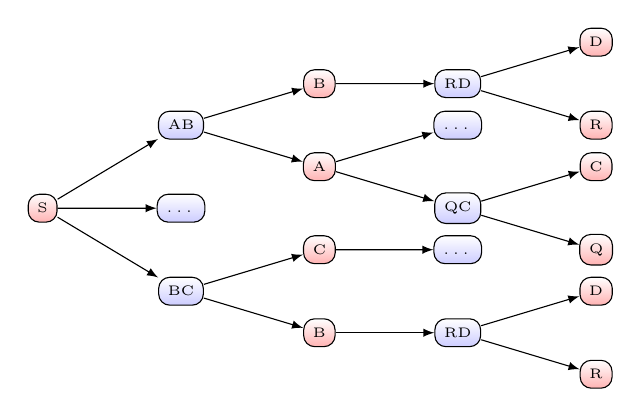
\begin{tikzpicture}
   [
     grow                    = right,
     sibling distance        = 3em,
     level distance          = 5em,
     edge from parent/.style = {draw, -latex},
     every node/.style       = {font=\footnotesize},
     sloped,
     treenode/.style = {shape=rectangle, rounded corners,
     draw, align=center,
     top color=white, bottom color=blue!20},
     root/.style     = {treenode, font=\tiny, bottom color=red!30},
     env/.style      = {treenode, font=\tiny},
     dummy/.style    = {circle,draw}
   ]
    \node [root] {S}
    child { node [env] {BC}
      child { node [root] {B}
        child { node [env] {RD}
          child { node [root] {R} }
          child { node [root] {D} }
        }
      }
      child { node [root] {C}
        child { node [env] {$\ldots\vphantom{BB}$} }
      }
    }
    child { node [env] {$\ldots\vphantom{BB}$} }
    child { node [env] {AB}
      child { node [root] {A}
        child {
          node [env] {QC}
          child { node [root] {Q} }
          child { node [root] {C} }
        }
        child { node [env] {$\ldots\vphantom{BB}$} }
      }
      child { node [root] {B}
        child { node [env] {RD}
          child { node [root] {R}  }
          child { node [root] {D}  }
        }
      }
    };
    \end{tikzpicture}
    }
    \caption{A partial $\mathbb{T}_2$ corresponding to the grammar $\{S \rightarrow BC \mid \ldots \mid AB, B\rightarrow RD \mid \ldots, A\rightarrow QC \mid \ldots\}$.}
    \label{fig:ptree}
    \vspace{-12pt}
  \end{wrapfigure}

  We will now describe a datatype for compactly representing CFL parse forests, then redefine the matrix algebra over this domain. This datatype is particularly convenient for tracking provenance under ambiguity, constructing the Parikh map for a CFG, counting the size of a finite CFL, and sampling parse trees with or without replacement.

  We first define a datatype $\mathbb{T}_3 = (V \cup \Sigma) \rightharpoonup \mathbb{T}_2$ where $\mathbb{T}_2 = (V \cup \Sigma) \times (\mathbb{N} \rightharpoonup \mathbb{T}_2\times\mathbb{T}_2)$\footnote{Given a $T:\mathbb{T}_2$, we may also refer to $\pi_1(T), \pi_2(T)$ as $\texttt{root}(T)$ and $\texttt{children}(T)$ respectively.}. Morally, we can think of $\mathbb{T}_2$ as an implicit set of possible trees that can be generated by a CFG in CNF, consistent with a finite-length porous string. Structurally, we may interpret $\mathbb{T}_2$ as an algebraic data type corresponding to the fixpoints of the following recurrence, which tells us each $\mathbb{T}_2$ can be a terminal, or a nonterminal and a (possibly empty) sequence of nonterminal pairs and their two children:\vspace{-10pt}

  \begin{equation}
    L(p) = 1 + p L(p) \phantom{addspace} P(a) = \Sigma + V L\big(V^2P(a)^2\big)
  \end{equation}

  Depicted in Fig.~\ref{fig:ptree} is a partial $\mathbb{T}_2$, where red nodes are \texttt{root}s and blue nodes are \texttt{children}. The shape of type $\mathbb{T}_2$ is congruent with an acyclic CFG in Chomsky Normal Form, i.e., $\mathbb{T}_2\cong\mathcal{G}'$, so assuming the CFG recognizes a finite language, as is the case for $G_\cap'$, then it can be translated directly. Since the RHS of CNF productions must be nonterminals, we define $P(a)$ as $\Sigma + V L\big(V^2P(a)^2\big)$, otherwise, we could write $\Sigma + VL\big(P(a)^2\big)$ to allow productions containing mixed $\Sigma$ and $V$.

  It is also possible to construct $\mathbb{T}_2$ for infinite languages by using the matrix fixpoint technique. If the CFG is cyclic, we can slice the language, $\mathcal{L}(G)\cap \Sigma^n$, and solve the fixpoint for each slice $n \in [2, n]$. Given a porous string $\sigma: \underline\Sigma^n$ representing the slice, we construct $\mathbb{T}_2$ from the bottom-up, and read off structures from the top-down. Here, we define first upper diagonal $\hat\sigma_r = \Lambda(\sigma_r)$ as:

\vspace{-5pt}\begin{equation}
  \begin{footnotesize}
\Lambda(s: \underline\Sigma) \mapsto \begin{cases}
\bigoplus_{s'\in \Sigma} \Lambda(s') & \text{if $s$ is a hole,} \vspace{5pt}\\
\big\{\mathbb{T}_2\big(w, \big[\langle\mathbb{T}_2(s), \mathbb{T}_2(\varepsilon)\rangle\big]\big) \mid (w \rightarrow s)\in P\big\} & \text{otherwise.}
\end{cases}
  \end{footnotesize}
\end{equation}

\noindent This initializes the superdiagonal entries of $M_0$, enabling us to compute the fixpoint $M_\infty$ in the same manner described in \S~\ref{sec:matrix_parsing}, by redefining $\oplus, \otimes: \mathbb{T}_3 \times \mathbb{T}_3 \rightarrow \mathbb{T}_3$ as:

\vspace{-5pt}\begin{align}
  X \oplus Z &\mapsto \bigcup_{\mathclap{k\in \pi_1(X \cup Z)}}\Big\{\phantom{.}k \Rightarrow \mathbb{T}_2(k, x \cup z) \mid x \in \pi_2(X\circ k), z \in \pi_2(Z\circ k)\phantom{.}\Big\}\\
  X \otimes Z &\mapsto \bigoplus_{\mathclap{(w\rightarrow xz) \in P}}\Big\{\phantom{.}\mathbb{T}_2\Big(w, \big[\langle X\circ x, Z\circ z\rangle\big]\Big) \mid x \in \pi_1(X), z \in \pi_1(Z)\phantom{.}\Big\}
\end{align}

These operators group subtrees by their root nonterminal, then aggregate their children. Instead of tracking sets, each $\Lambda$ now becomes a dictionary of $\mathbb{T}_2$, indexed by their root nonterminals. This ensures each matrix entry $\Lambda_{i,j}$ contains at most $|V|$ separate $\mathbb{T}_2$ instances, each representing a reachable nonterminal and all possible ways to derive that nonterminal from $\sigma_{i..j}$, i.e., all parse forests sharing the same root, consistent with the porous substring in the first upper diagonal.

\clearpage